%% The following is a directive for TeXShop to indicate the main file
%%!TEX root = ../../thesis.tex

\chapter{Open source practices for education}
\label{app:education}

\section{Introduction}
Just as visualizing and interacting with simulation results is useful in a research context, it can be a powerful mechanism by which learners can build their understanding on concepts in geophysics. With the availability of tools such as Jupyter \citep{Perez2015}, as well as platforms like Binder \citep{ProjectJupyter2018} which provide hosting and computational resources, software developed in a research context can be readily re-purposed and used in a teaching context. Much of the difference between learning in an educational context and learning in a research context is essentially whether the concepts being learned are well-established in the field, or at the edge of our knowledge. As such, a common set of tools can be used to serve both purposes.

Beyond the ability to interact with content, hosting resources on the web provides the opportunity for multiple contributors to be involved in the development, maintenance and curation of the resources. Unlike print textbooks, which are static, open-source web based resources can be continually updated as mistakes are found, new examples generated and explanations improved. Further, there are a host of tools within the open source software ecosystem that enable interactive content, which connect computation to images and explanations, to be built.

In the GeoSci.xyz project (\href{https://geosci.xyz}{https://geosci.xyz}), we have been working to take practices for open-source software development and apply them to the development of educational resources. GeoSci.xyz is a collection of collaboratively developed resources for research and education in the geosciences. To date, it includes three modules that each have ``textbook'' component and a collection of Jupyter-notebook apps associated with them:
\begin{itemize}
    \item GPG: Geophysics for practicing geoscientists (\href{https://gpg.geosci.xyz}{https://gpg.geosci.xyz})
    \item EM: Electromagnetic geophysics (\href{https://em.geosci.xyz}{https://em.geosci.xyz})
    \item Toolkit: Geophysical toolkit for geologists (\href{http://toolkit.geosci.xyz}{http://toolkit.geosci.xyz})
\end{itemize}

The GPG is targeted at the undergraduate level and provides introductory material and an overview of the physical principles governing geophysical methods including magnetics, seismic, ground penetrating radar and electromagnetics. This is used as the primary textbook in the course EOSC 350: \emph{Environmental, Geotechnical and Exploration Geophysics I} offered at the University of British Columbia.

The EM module is an in-depth resource for electromagnetics. It covers fundamentals, starting at Maxwell's equations, through to the suite of electromagnetic geophysical techniques (e.g. DC resistivity, Induced Polarization, Airborne Electromagnetics, …). It also includes case-histories which methodically walk through an application of electromagnetics to answer a geoscientific question. In 2017, the Society of Exploration Geophysics Distinguished Instructor Short Course (SEG DISC) on \emph{Geophysical Electromagnetics: Fundamentals and Applications} was given by Dr. Douglas Oldenburg, myself and Dr. Seogi Kang; em.geosci.xyz served as the main resource for participants.

The Toolkit is the most recent addition to the GeoSci.xyz ecosystem. This module is the result of a collaborative project between the Mineral Deposits Research Unit (MDRU) and the Geophysical Inversion Facility (GIF) at the University of British Columbia. It is intended to be a resource for geologists who are interested in incorporating geophysical data into their interpretation workflow. The main focus is on techniques for incorporating magnetic data into a geologic interpretation.

Each of the GeoSci.xyz modules bring together text, images, software, live-computation and practices from open source software development to create training and educational resources. The contents is open-source, licensed under the Creative Commons Attribution 4.0 International (CC BY 4.0) license which allows reuse and adaptation of the content. The development and maintenance of these resources follows open development practices including version control, issue tracking, and testing. Suggested edits and enhancements to the resources can be made by anyone, and all content additions or changes are peer-reviewed prior to updating each module. Source-code used to generate figures is captured with those figures; it is tested upon each update to any of the modules and accessible to users so that they can reproduce the results or change the inputs. These same codes are connected are used to generate ``apps'' using Jupyter notebooks and the ipywidgets package which allow users to interact with a numerical simulations through slide-bars and toggle buttons.

This appendix provides an overview of the underlying technology and some of the implications of capturing content in a modern, web-based framework that interoperates with open-source software. Section \ref{sec:geosci-textbooks} discusses the technology used to build the ``textbook'' component of each of the modules, including how source-code is captured to ensure figures are reproducible. Section \ref{sec:interactive} demonstrates how Jupyter notebooks are used to make interactive content that connects live numerical simulations with widgets and visualizations. Finally, Section \ref{sec:open-development} discusses open development practices including peer-review, testing, and collaboration.

\section{GeoSci.xyz Textbooks}
\label{sec:geosci-textbooks}

More than two decades ago, \cite{Claerbout1992} articulated the potential for using web-technology to improve reproducibility, particularly of computational work. Since then, the open-source software ecosystem has grown significantly. As a result, there a many more high-quality tools that are freely available and interoperable with one another, simplifying the task of creating reproducible web-based content.

All of the GeoSci.xyz content is hosted and maintained on GitHub (\href{https://github.org/geoscixyz}{https://github.org/geoscixyz}). The GeoSci.xyz modules leverage a common python documentation generator, Sphinx (\href{http://sphinx-doc.org}{http://sphinx-doc.org}), to build the websites. Each site is built and maintained as a collection of simple text-files that are compiled to the html website that users see. The pages can be edited in any text editor or directly on GitHub.

There are several Sphinx-extensions which we make use of in order to capture scientific content, including to manage bibliographies and to create plots from code. Figure \ref{fig:reproducible_figure} shows a page on \href{em.geosci.xyz}{em.geosci.xyz} that discusses the solution for a conductive sphere in a whole-space subject to a uniform electric field. The plot compares total and secondary electric fields for both conductive and resistive spheres. This plot is built from Python code; the text-file from which this page is built is shown in Figure \ref{fig:reproducible_figure_source}. Rather than storing the image file, the source- code is written into the page and compiled when the site is built. In this way, readers can always access the source code, and engaged readers can download the code, update the input parameters, run the computation, and explore the impact on the resultant image. In terms of maintenance, if errors are found in the computation or mistakes in labels or annotations of the figure, the source code can be altered and the figure rebuilt.

\begin{figure}
    \begin{center}
    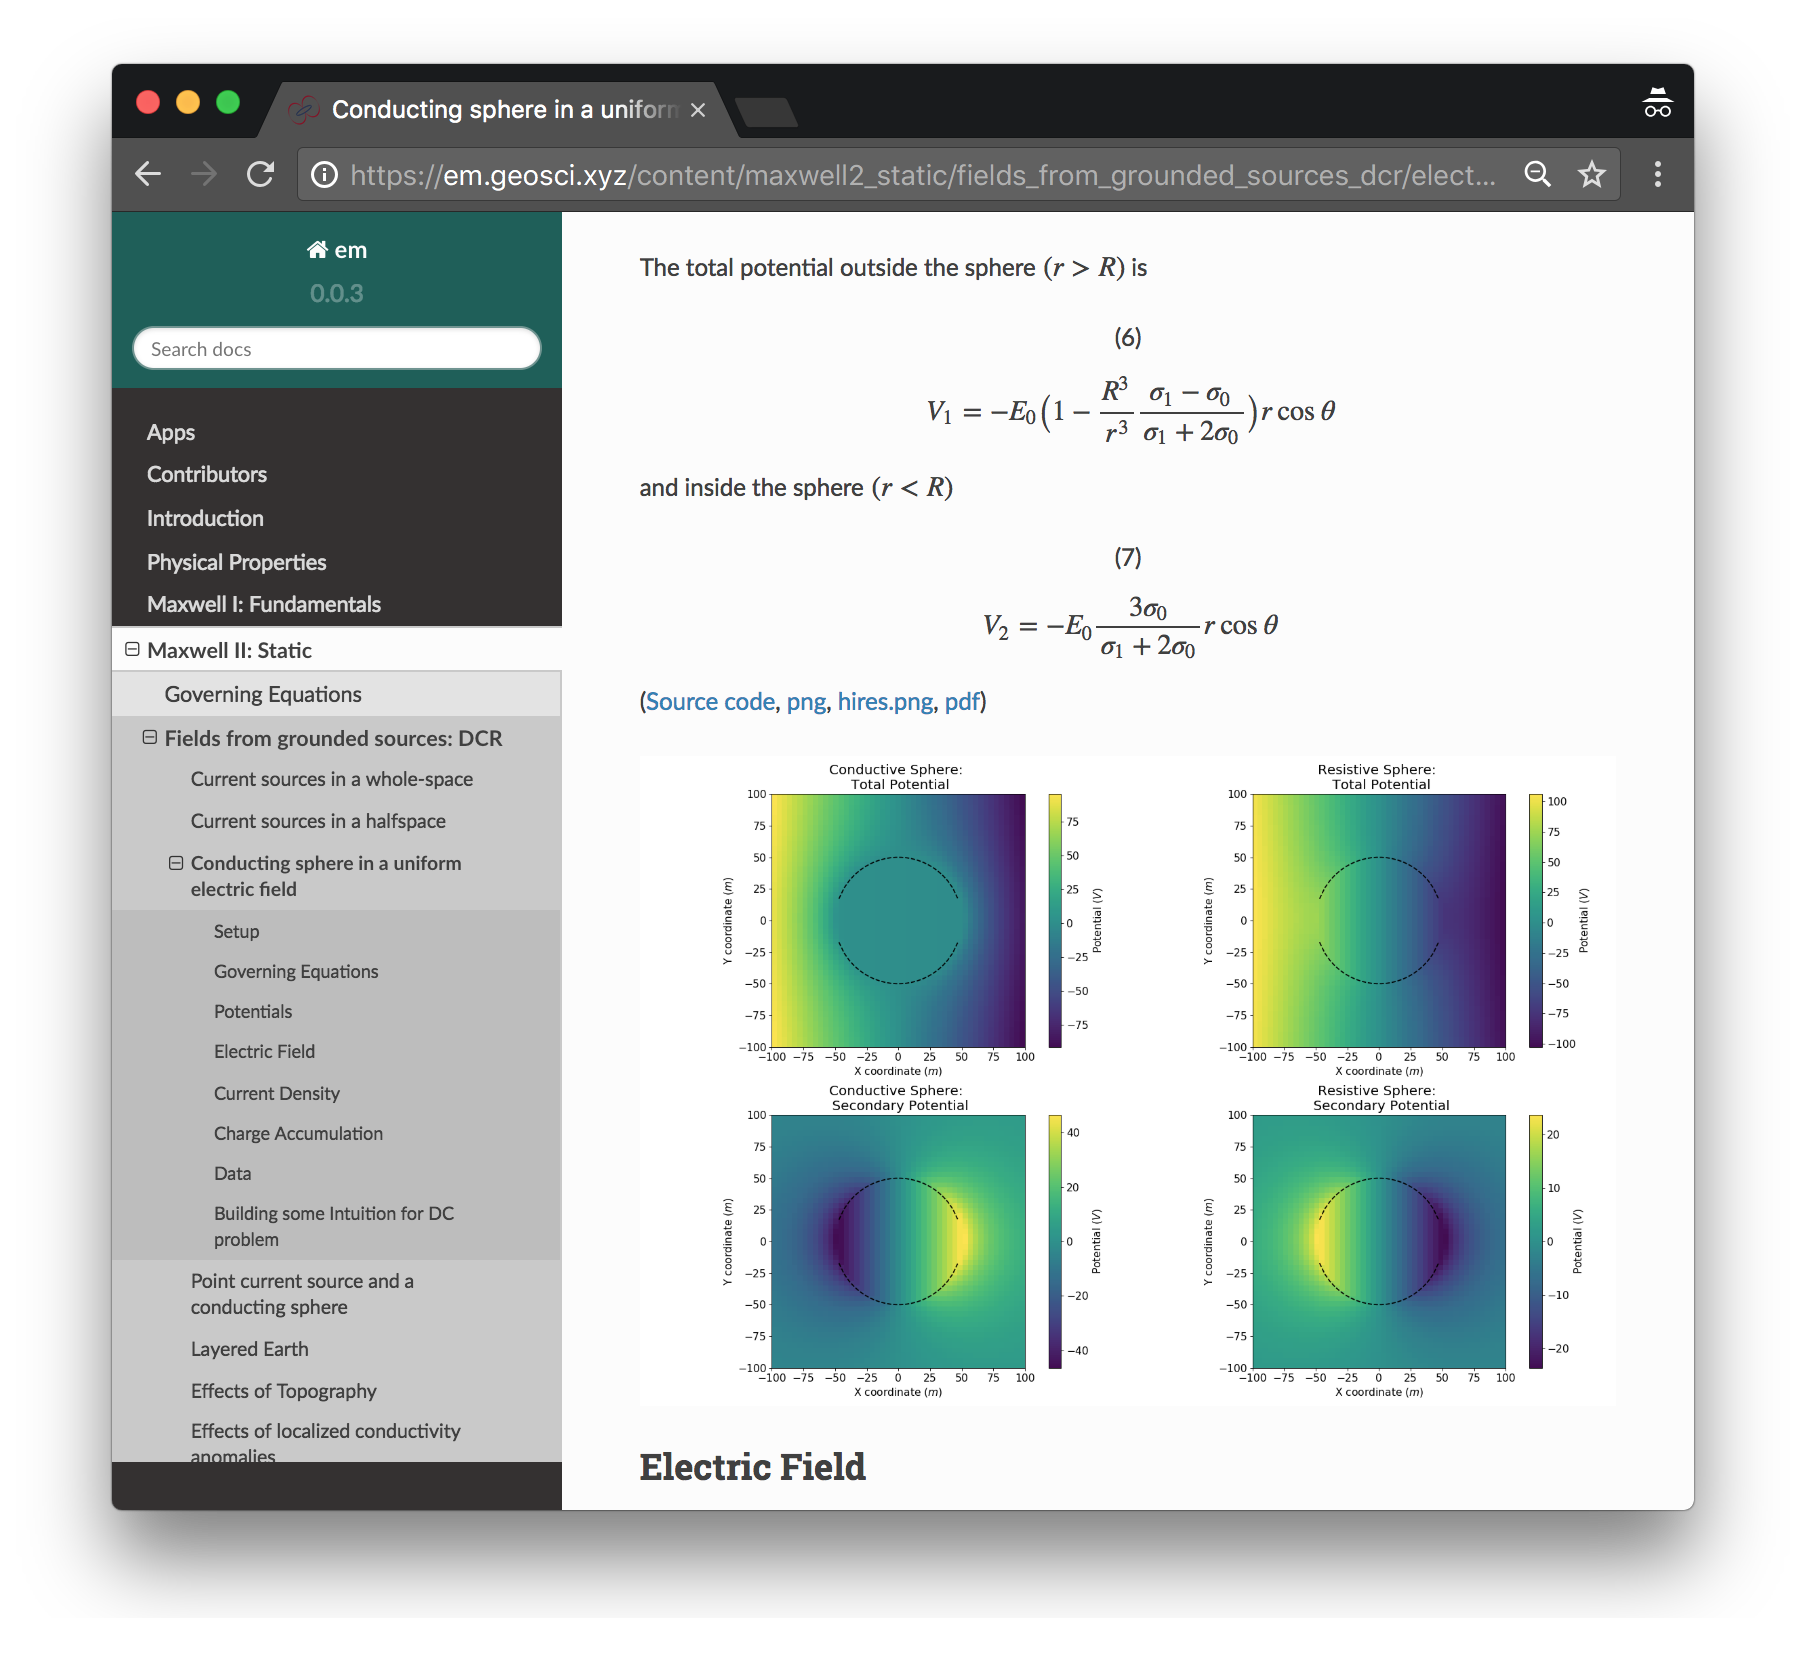
\includegraphics[width=\textwidth]{figures/education/reproducible_figure.png}
    \end{center}
\caption{
    Web-page on a conducting sphere in a uniform electric field
    (\href{https://em.geosci.xyz/content/maxwell2_static/fields_from_grounded_sources_dcr/electrostatic_sphere.html}{https://em.geosci.xyz/content/maxwell2\_static/fields\_from\_grounded\_sources\_dcr /electrostatic\_sphere.html}).
    The plot shown on this page is compiled from Python code and can be downloaded and run by users, or update by maintainers if there are improvements that can be made.
}
\label{fig:reproducible_figure}
\end{figure}





\begin{figure}
    \begin{center}
    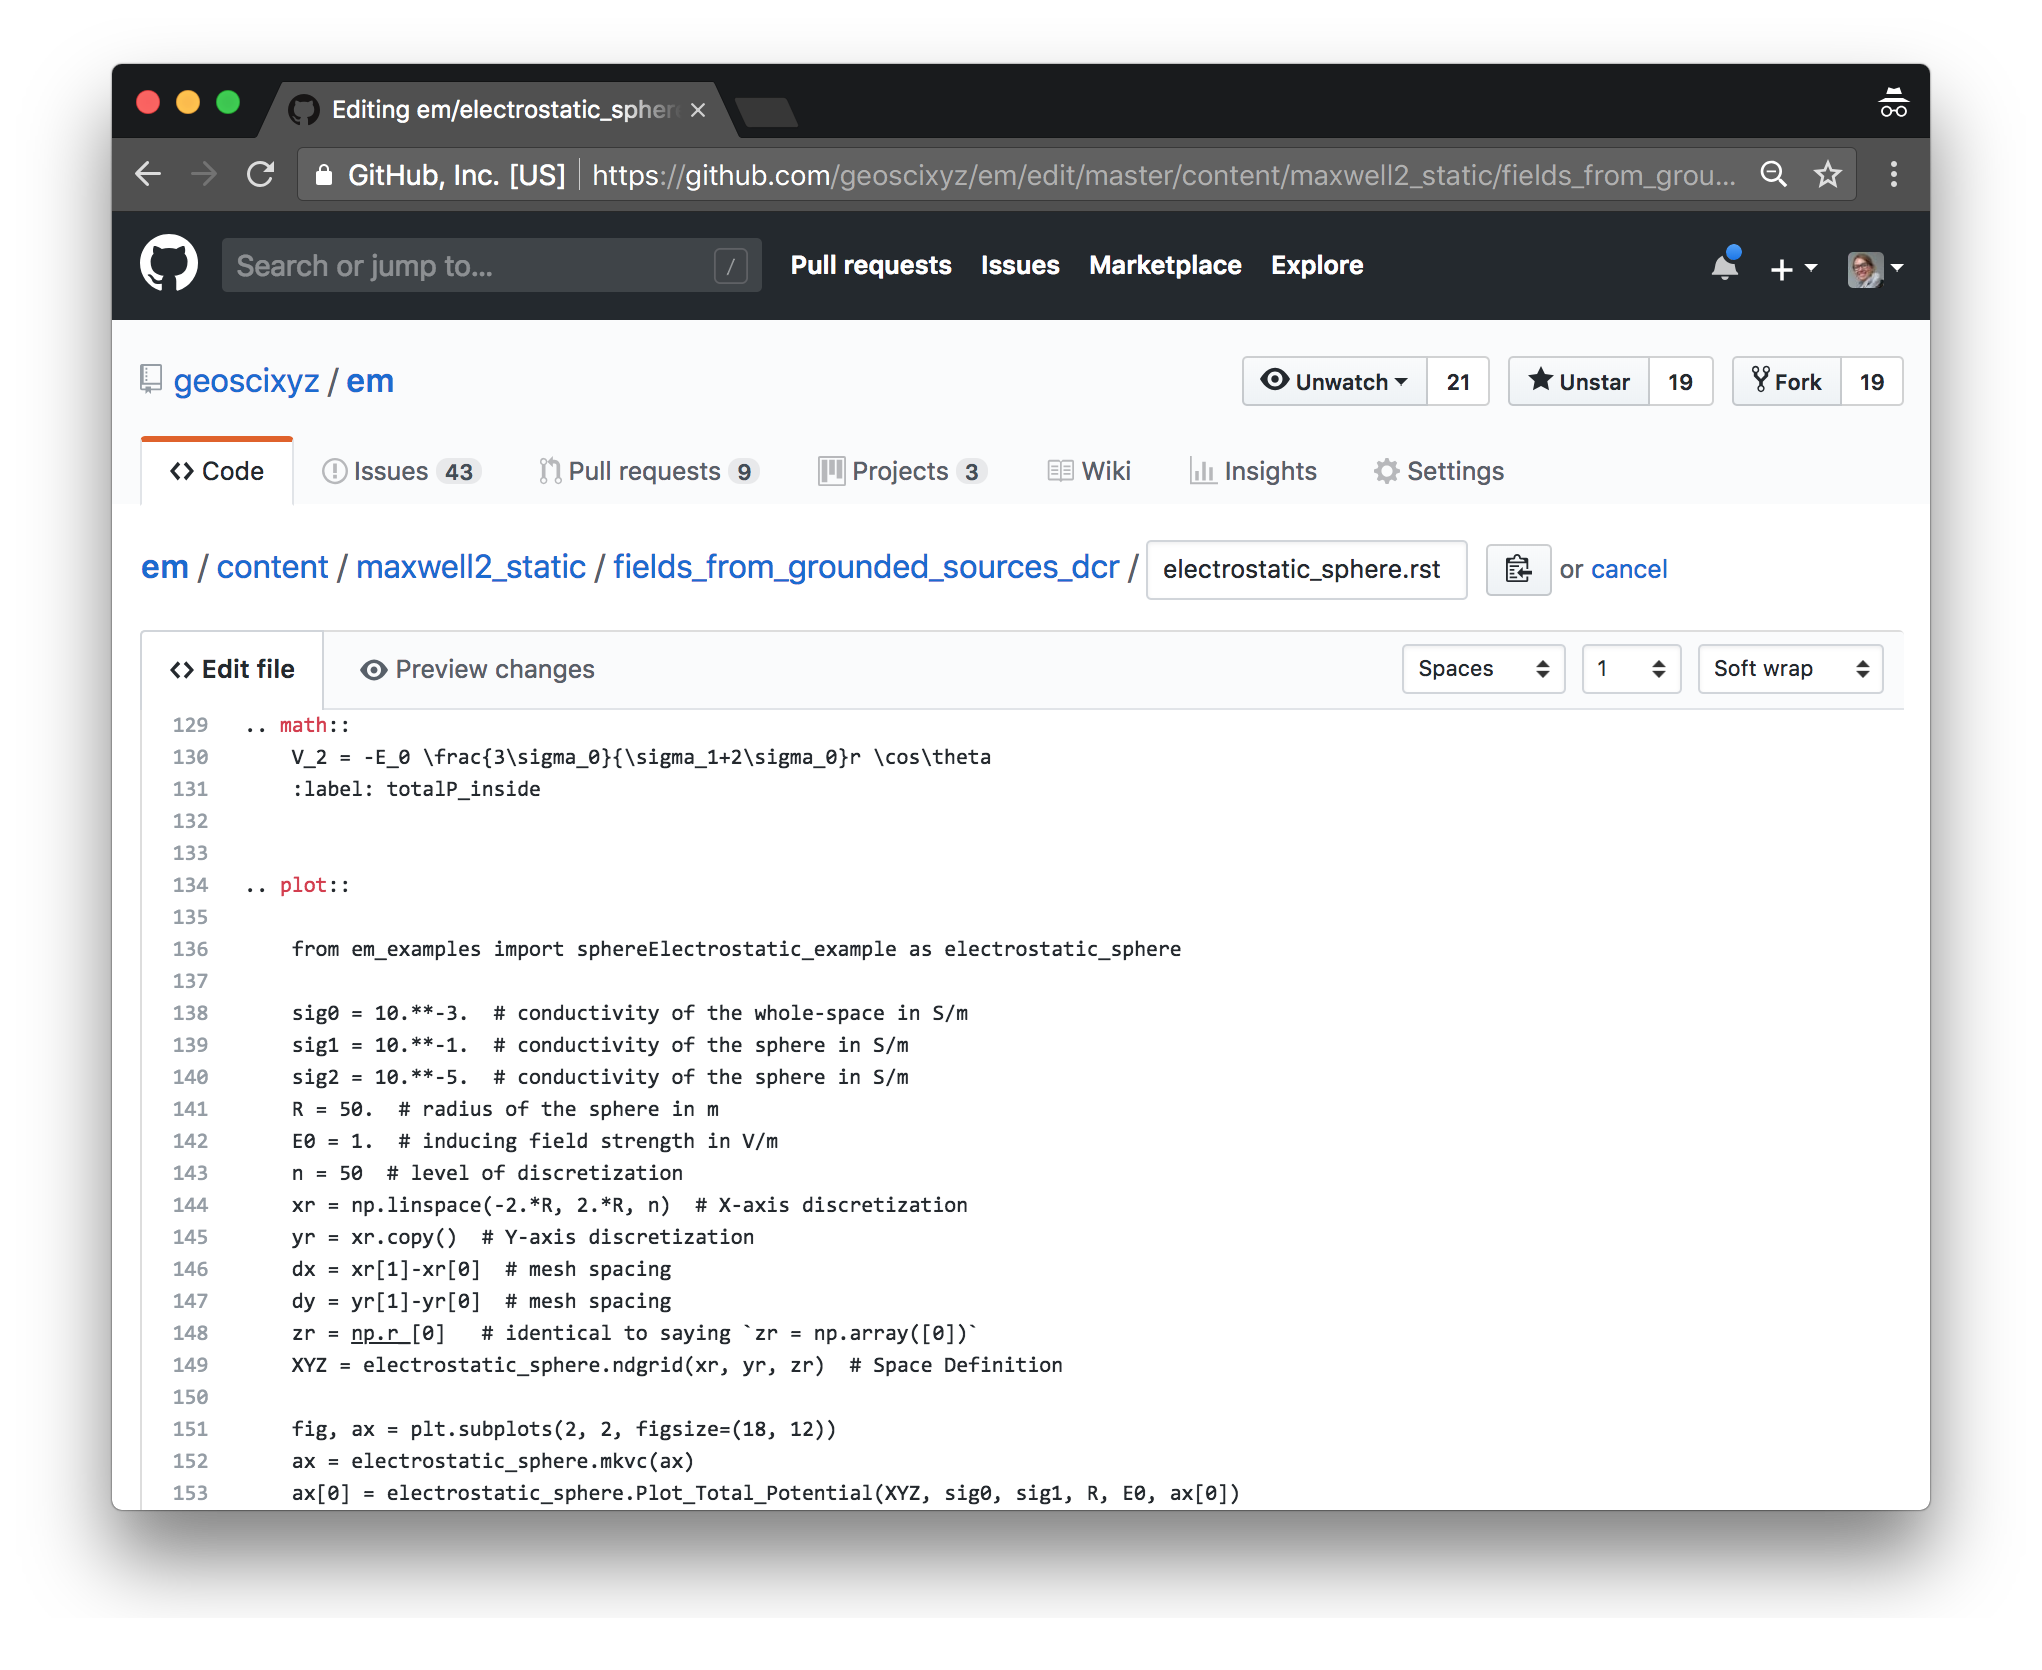
\includegraphics[width=\textwidth]{figures/education/reproducible_figure_source.png}
    \end{center}
\caption{
    Text source from which the web-page shown in Figure \ref{fig:reproducible_figure} is built.
    The code used to build the plot starts under the plot-directive on line 134.
}
\label{fig:reproducible_figure_source}
\end{figure}





Simple sites, without intensive computation can be hosted on the free documentation hosting service ReadTheDocs (\href{https://readthedocs.org}{https://readthedocs.org}). Several of the examples on the GeoSci.xyz sites involve simulations of Maxwell's equations, and have thus exceeded the resource limits on ReadTheDocs, so instead we build the modules on a continuous integration service and deploy to a Google App Engine website.

\section{Interactive content}
\label{sec:interactive}

Static figures can be made dynamic and interactive by connecting them with a live computational environment. The Jupyter Notebook combines text, images, lines of code, outputs and interactive widgets into a single ``computational narrative'' \citep{Perez2015}. Much of the research conducted in this thesis relied on Jupyter Notebooks and benefited from the iterative workflow it supports as well as the widget architecture that allows computation to be connected to visualization through slide-bars and toggle buttons. Millions of researchers, data analysts, and journalists have adopted the Jupyter notebook (or similar computational notebooks) as a tool for authoring computational workflows and analyses \citep{Rule2018}.

The ability to include narrative text to document a workflow, visualize results inline, and conduct iterative analyses are all reasons that the Jupyter Notebook is a valuable research tool. For many of the same reasons, it is a powerful medium for developing and delivering educational content. Text which provides instructions or prompts questions to guide a learner can be included in the Notebook and provide context for the ``app'' or simulation tool. Depending on the purpose of the exercise, lines of code can be displayed, for example if the aim of the exercise is to walk through how to discretize the DC resistivity problem. Alternatively, if the physics is the central focus, the code can be abstracted-away, and the learner provided with widgets to run a simulation (see Figure \ref{fig:jupyter-app}).


\begin{figure}
    \begin{center}
    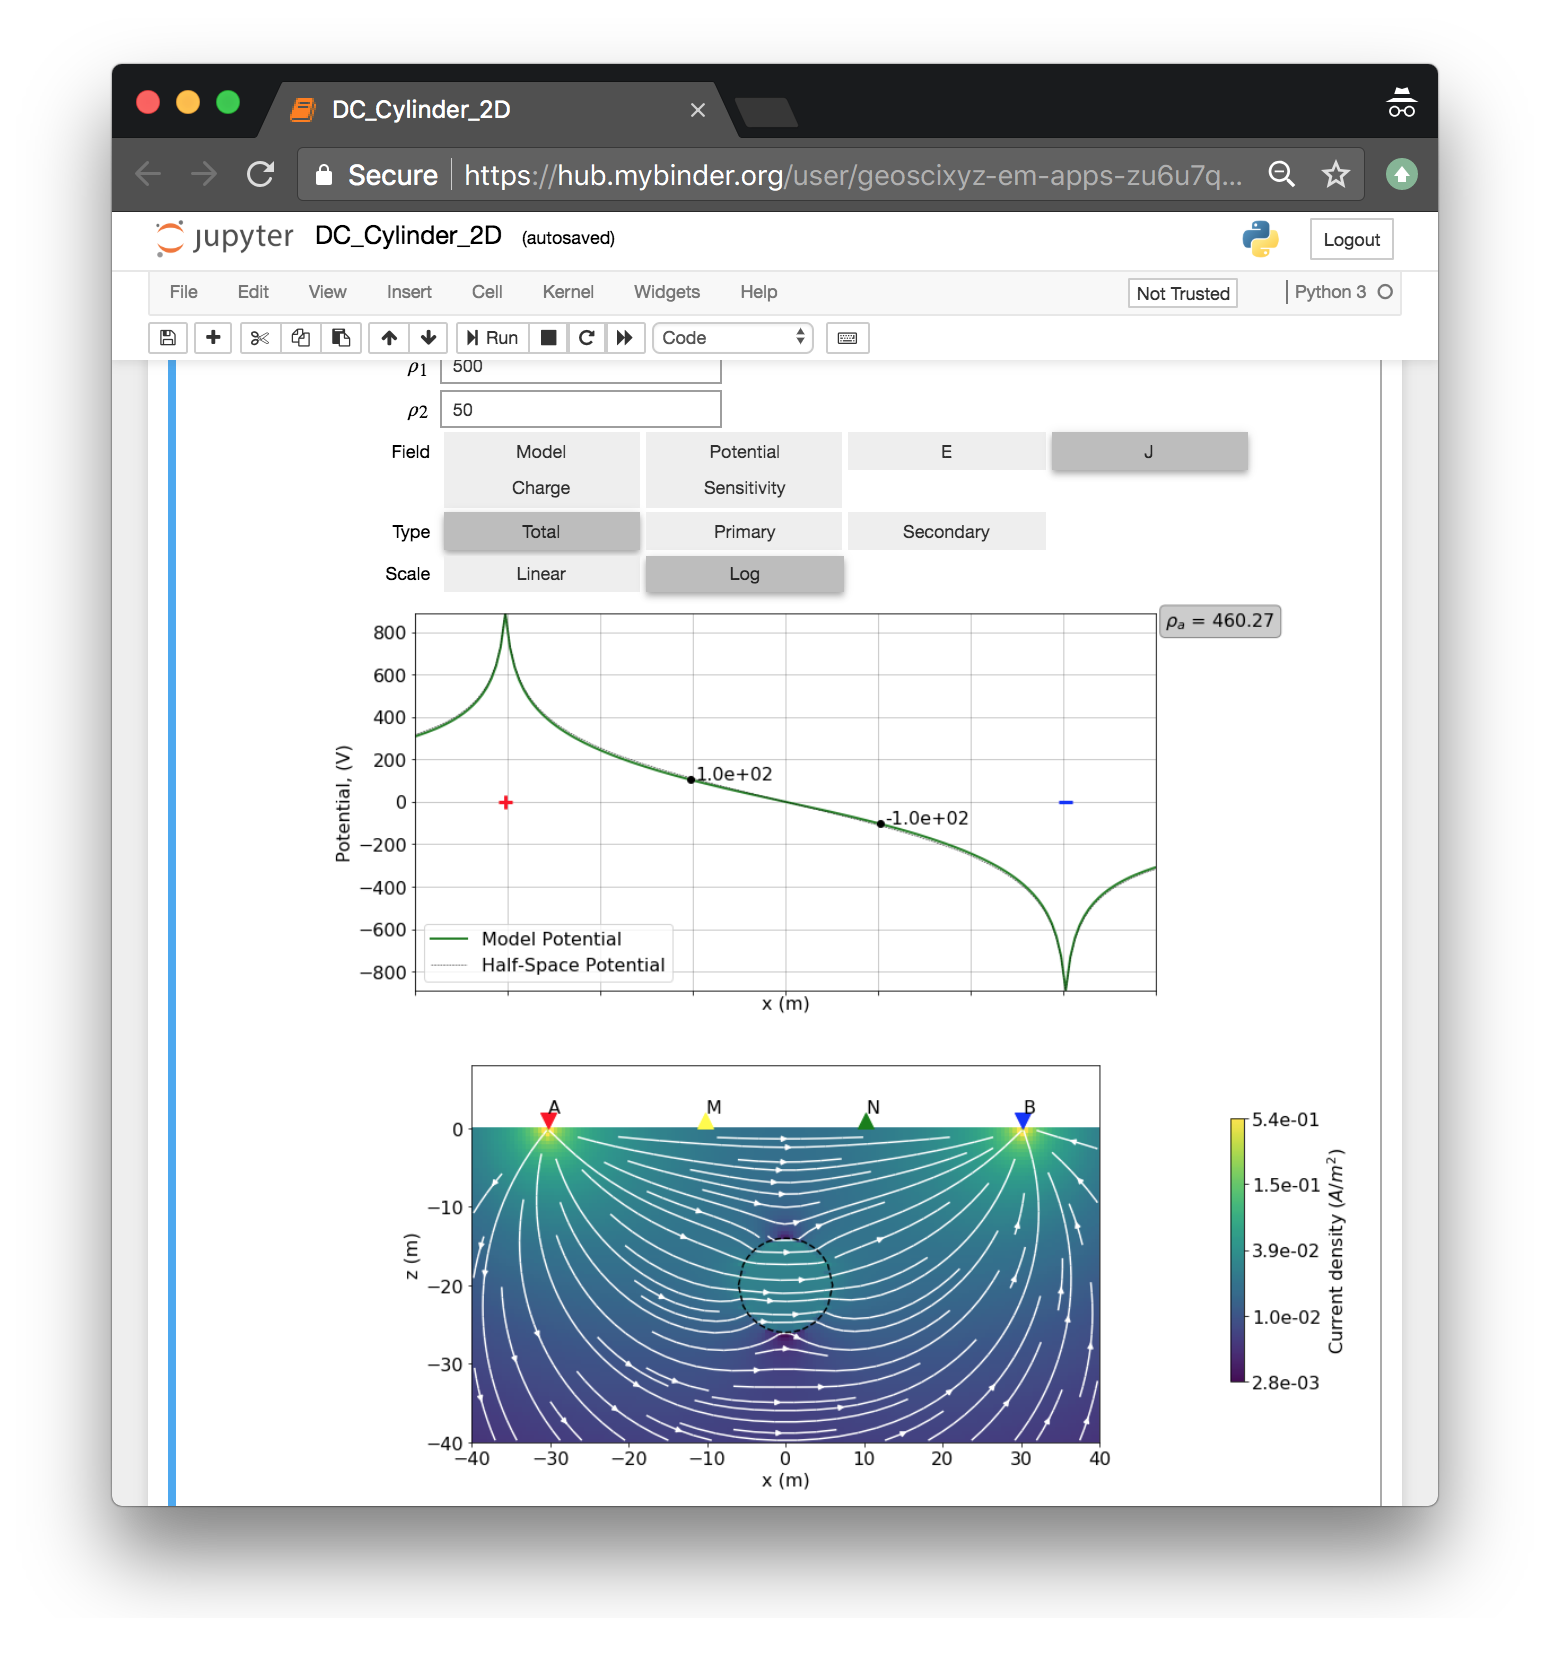
\includegraphics[width=\textwidth]{figures/education/jupyter-app.png}
    \end{center}
\caption{
   A sample Jupyter notebook ``app'' that simulates a DC resistivity over a halfspace
   with a cylinder. The widgets control the visualization. The user can change the model parameters
   (e.g. the resistivity of the cylinder and of the background), the survey geometry, and select the visualization
   (e.g. electric field, currents, charges, etc.)
}
\label{fig:jupyter-app}
\end{figure}





To date, there are 17 Notebooks associated with the GPG, $>$ 30 with the EM module, and 10 for the Toolkit. We provide instructions for downloading the Notebooks and setting up the necessary software environment to run them. However, many of the learners we are working to reach are not necessarily familiar with setting up a software environment or launching applications from the command-line, and so these steps present a significant overhead. To overcome this barrier, we use Binder (\href{http://mybinder.org}{http://mybinder.org}, \cite{ProjectJupyter2018}), which is a web-service that provides cloud-based hosting of Jupyter notebooks. As notebook authors, we provide the set of dependencies required to run the notebooks, and these are automatically installed when the user follows the Binder-url to the notebooks. The user is then served the Notebook in a live computational environment that is accessed from their web-browser. Using services like Binder means that learners do not need to open a command-prompt nor do they need to be familiar with how to manage a software environment. The focus then, can remain on the content.

Using Jupyter Notebooks as the medium for authoring educational content has the added benefit that many researchers and graduate students are already familiar with Notebooks. The simulation tools and tutorials are built on research code such as SimPEG, that are already a part of many of the contributors research toolbox. This removes the need for contributors to learn a new set of tools for the sole purpose of sharing educational content. In the long-run, we hope that by bringing research codes into education, engaged learners then have a trajectory to move beyond using the ``apps'' for learning a concept in geophysics and can further explore the computational steps taken to run those same simulations.
\section{Open development}
\label{sec:open-development}

Best practices in open-source software development have enabled the growth and maintenance of software tools for that support large communities of researchers (e.g. Astropy in astronomy \citep{Astropy2013}, SciPy in scientific computing \cite{scipy}). In many of these projects, it is a handful of ``core developers'' who are responsible for generating the majority of the software, but each benefits from the minor enhancements, bug-fixes, and additions made by the ``long tail'' of contributors. In contrast, most educational resources are authored and maintained by a individual instructors. There is minimal opportunity for feedback or improvements to be made by others in a scalable way. Seeing the success of the open-source software ecosystem, we have sought to adopt many of the same practices in the hopes of fostering a community of educators and learners around open-source educational material. This section outlines some of those practices.

Modern version control using git and GitHub (or similar) is an essential tool for allowing multiple contributors to productively work on different aspects of a project and have their improvements incorporated back into the main project. New content or edits on existing content incorporated into the module through a pull-request process. A pull-request shows a comparison between the main version of the module and the version containing the suggested changes and provides the opportunity for peer-review. Suggested changes to any of the GeoSci.xyz modules are peer-reviewed on GitHub prior to being merged into the main version of the module. Each web-page in the GeoSci.xyz textbooks has an ``edit on GitHub'' button that allows anyone to edit the current page and submit a pull request for their edits to be included in the live-site.

Issue trackers are used in software projects to notify developers of bugs that are found in the software and to keep track of the progress of a bug-fix, or similarly, to submit and track feature requests. The same concepts can be applied to the development of educational content. For example, some mathematical typos are subtle and require discussion to sort-out; prior to suggesting an edit, a contributor might create an issue to prompt that discussion.

When multiple contributors are working on a single code-base, testing is important to ensure that changes do not break existing functionality. For the GeoSci.xyz textbook-modules, we test that the website comiles. This ensures that no syntax errors have been introduced into the text and that the code used to build the figures runs without error. We also test that all of the external links that the site points to for additional resources are valid. If, for some reason, a web-page that we were referencing is taken-down, the testing provides an alert and we can find a new resource or remove the broken link. All of the associated Jupyter notebooks are also tested. These tests execute all of the code in each of the notebooks and alert us if any errors are raised. Each of the GeoSci.xyz modules is tested on a monthly basis using TraviCI (\href{https://travis-ci.org/}{https://travis-ci.org/}), a continuous integration and testing service that is free for open source projects. This ensures that the website continues to compile and provides alerts if there have been changes in upstream software dependencies that cause any computations included in the resource to fail.

In addition to the practices state above, there are also best practices that can be learned from a well-architected code-base. Aspects of a well-designed code-base include modularity and the use of inheritance to promote a consistent structure across the project. If a software package is well-structured and well-organized, it becomes easier to invite contributors as it is evident where their contribution fits into the project. The case-histories in em.geosci.xyz are one place where we have used the concept of inheritance, in which a base-class provides the outline or template of the content, to provide structure. Each case history is structured in seven steps, as shown in Figure \ref{fig:seven_steps}. As a contributor, this is a well-structured template that can be followed and filled-in. As a learner, this structure provides consistency across content that is contributed by multiple authors and a framework in which to organize concepts.


\begin{figure}
    \begin{center}
    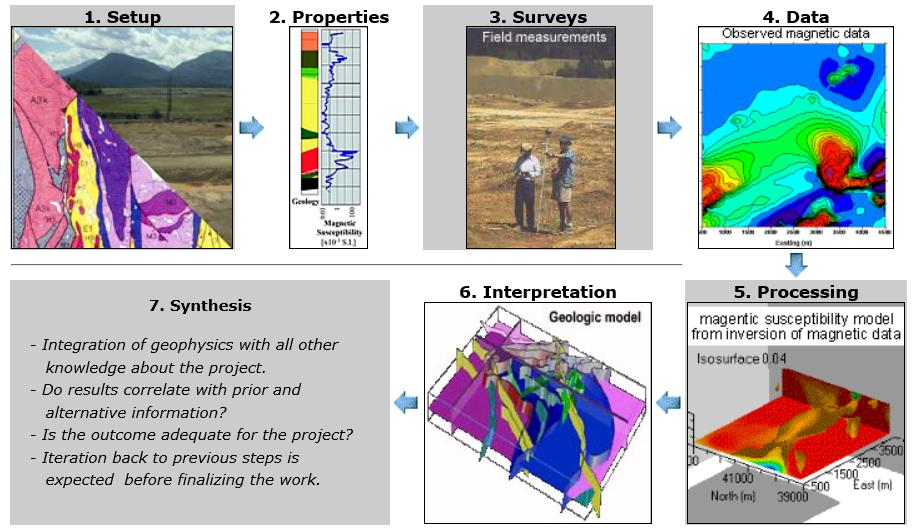
\includegraphics[width=0.8\textwidth]{figures/education/seven_steps.jpg}
    \end{center}
\caption{
   Seven step framework used for the case histories in \href{https://em.geosci.xyz}{https://em.geosci.xyz}.
   (1) Setup: describe the geoscientific question and objectives that are to be addressed.
   (2) Properties: identify the diagnostic physical properties (e.g. density, electrical conductivity, magnetic susceptibility, etc.).
   (3) Survey: design a survey that is suitable for detecting the physical property contrasts relevant to the application.
   (4) Data: carry out the field survey and collect the data set(s).
   (5) Processing: plot the data and apply the analysis steps needed to interpret the data (e.g. invert the data).
   (6) Interpretation: interpret the results in terms of the identified physical properties and original geoscience objective.
   (7) Synthesis: integrate the interpretation with geologic and other information relevant to the application in order to address the original geoscience objective.
   This image and caption are adapted from:
   \href{https://em.geosci.xyz/content/geophysical_surveys/fundamentals/seven_steps.html}{https://em.geosci.xyz/content/geophysical\_surveys/fundamentals/ seven\_steps.html}
}
\label{fig:seven_steps}
\end{figure}




\section{Conclusions and outlook}

Applied geophysics is a relatively small community. There are not many methods-oriented textbooks or resources available. As a result there is significant duplication of efforts as many educators develop their own set of resources, often in isolation. Even if these resources are captured and made available in the form of a textbook, the content rapidly becomes out-of-date as instrumentation and data analyses techniques continually improve. An open-source approach to the development of software has enabled widespread collaboration on the tools that support communities of researchers. Our hope is that an open-source approach to the development of educational resources can catalyze a similar community in the geosciences.
